\documentclass[a4paper,12pt]{article}

\usepackage{ucs}
\usepackage[utf8x]{inputenc}
\usepackage[russian]{babel}
\usepackage{graphicx}
\usepackage{listings}
\usepackage{xcolor}

\makeatletter
\renewcommand\@biblabel[1]{#1.}
\makeatother

\newcommand{\myrule}[1]{\rule{#1}{0.4pt}}
\newcommand{\sign}[2][~]{{\small\myrule{#2}\\[-0.7em]\makebox[#2]{\it #1}}}

% Поля
\usepackage[top=20mm, left=30mm, right=10mm, bottom=20mm, nohead]{geometry}
\usepackage{indentfirst}

% Межстрочный интервал
\renewcommand{\baselinestretch}{1.50}


\begin{document}

%%%%%%%%%%%%%%%%%%%%%%
%%%                %%%
%%% Титульный лист %%%

\thispagestyle{empty}
{ \large
\begin{center}
\renewcommand{\baselinestretch}{1.4}
Министерство науки и высшего образования Российской Федерации\\
\bigskip
Федеральное государственное бюджетное образовательное учреждение \\ 
высшего образования <<Петрозаводский государственный университет>>\\
\bigskip
Институт математики и информационных технологий \\
кафедра информатики и математического обеспечения

\end{center}
}
\vspace{3\bigskipamount}%

\vspace{2\bigskipamount}

\begin{center}
\large
Плугин Олег Антонович
\end{center}
\medskip%

%%% Название работы %%%
\begin{center}
\renewcommand{\baselinestretch}{1.2}
\Large \sc Разработка модели распознавания автомобильных номеров на основе технологий компьютерного зрения
\end{center}
\medskip%


\begin{center}
\large
ВЫПУСКНАЯ КВАЛИФИКАЦИОННАЯ РАБОТА
\end{center}
\medskip%

\begin{center}
\large
Направление подготовки бакалавра \\
09.03.02 - Информационные системы и технологии \\
Форма обучения - очная
\end{center}

\vspace{4\bigskipamount}%

\begin{tabular}{ l l }
    Допущена к защите. & \\
    Заведующий кафедрой, & \hspace{2cm} Руководитель \\
    кандидат технических наук & \hspace{2cm} \parbox[t]{6cm}{кандидат физико-математических наук} \\
    Богоявленский Юрий Анатольевич & \hspace{2cm} Корзун Дмитрий Жоржевич \\
    \noindent\rule{6cm}{0.2pt} & \hspace{2cm} \noindent\rule{6cm}{0.2pt} \\
    <<\noindent\rule{1cm}{0.2pt}>>\noindent\rule{3cm}{0.2pt}202\noindent\rule{0.3cm}{0.2pt} г. & \hspace{2cm}
    <<\noindent\rule{1cm}{0.2pt}>>\noindent\rule{3cm}{0.2pt}202\noindent\rule{0.3cm}{0.2pt} г.
\end{tabular}

\vfill
\begin{center}
\large
Петрозаводск --- 2025
\end{center}


%%%%%%%%%%%%%%%%%%
%%%            %%%
%%% Содержание %%%
\newpage

\setcounter{tocdepth}{4}
\tableofcontents

%%%%%%%%%%%%%%%%
%%%          %%%
%%% ВВЕДЕНИЕ %%%

\newpage
\section*{Введение}
\addcontentsline{toc}{section}{Введение}

\textbf{Актуальность темы}

Системы автоматического распознавания различных объектов становятся неотъемлемой частью современных технологий. Они используются в самых разных сферах жизни, включая промышленность, медицину, транспорт и другие направления [1]. Такие системы позволяют автоматизировать процессы анализа изображений и видео, что позволяет распознавать лица, жесты и любые другие визуальные элементы.

Одним из примеров применения технологий распознавания является система распознавания автомобильных номерных знаков. Она активно внедряется на контрольно-пропускных пунктах, охраняемых территориях, платных парковках и дорогах общего пользования, т.к. на таких объектах требуется автоматическая идентификация транспортных средств [1].

Современные решения, основанные на на использовании нейросетей и методов компьютерного зрения, позволяют автоматизировать процессы, которые раньше производились вручную, при этом обеспечивая высокую точность, скорость и стабильность работы в различных условиях, включая плохую погоду, освещенность или низкое качество изображения. Системы, использующие такие решения, способны работать в круглосуточном режиме без снижения эффективности, обеспечивая непрерывную обработку потока данных, в отличие от человека.

Актуальность темы также обусловлена активным развитием технологий искусственного интеллекта и повышением интереса к задачам автоматизации различных систем. Разработка и исследование таких систем требует применения современных архитектур нейросетей, технологий оптического распознавания текста (OCR), и работой с большим объемом визуальных данных за счет использования компьютерного зрения. Это чётко закреплено в в государственной программе Российской Федерации "НАЦИОНАЛЬНАЯ СТРАТЕГИЯ  РАЗВИТИЯ ИСКУССТВЕННОГО ИНТЕЛЛЕКТА НА ПЕРИОД ДО 2030 ГОДА".

Предприятие ОАО "Петрозаводскмаш" выступает в роли инициатора проекта, т.к. возникла необходимость в системе автоматизированного контроля потока автомобилей, поступающего на частную парковку предприятия, обеспеченную системами видео-наблюдения.
Существующие решения не устроили руководство предприятия, так как являются экономически нецелесообразными в связи со своей высокой стоимостью использования, а также требованиями к вычислительной мощности оборудования. Открытые решения не удовлетворяют ожидаемой точностью, а также отсутствием возможности настройки под условия использования заказчиком.

\textbf{Цель и задачи работы}

Целью выпускной квалификационной работы является разработка программной системы, которая способна в автоматическом режиме определять регистрационные знаки транспортных средств на изображениях и распознавать текст, содержащийся на них, с использованием современных методов компьютерного зрения и машинного обучения.

Для достижения поставленной цели необходимо решить следующие задачи:
\begin{enumerate}
    \item Изучить теоретические основы компьютерного зрения, детекции объектов и оптического распознавания текста.
    \item Проанализировать существующие подходы и решения в области автоматического распознавания автомобильных номеров.
    \item Провести выбор и обоснование инструментов и программных библиотек, подходящих для реализации задачи.
    \item Подготовить и разметить датасет, объединив изображения из различных источников и приведя их к единому формату, подходящему использующейся модели.
    \item Обучить и дообучить модель для задачи детекции номерных знаков с использованием подготовленных данных.
    \item Интегрировать модель детекции с моделью распознавания текста.
    \item Провести тестирование системы для оценки точности работы модели распознавания.
    \item Проанализировать оценку работы и рассмотреть возможные варианты дальнейшего улучшения системы.
\end{enumerate}

\textbf{Предмет исследования}

Предметом исследования в работе являются методы и технологии детекции и распознавания текста на изображениях с помощью технологий компьютерного зрения. Эти методы служат инструментом для идентификации автомобильных номеров транспортных средств.
Особое внимание уделяется различным архитектурам нейронных сетей, которые позволяют производить обнаружение объектов, а также распознавание символов изображений и преобразование их в текстовый вид, являющиеся претендентами на возможное использование в практической реализации системы.

\textbf{Методы исследования}

В работе используются следующие методы исследования:

\begin{itemize}
    \item \textbf{Анализ и сравнение} уже существующих решений в области распознавания регистрационных знаков автомобилей для российских и зарубежных авто мномеров
    \item \textbf{Методы машинного обучения}, которые основаны на архитектуре сверточных нейросетей, используемых в реализации системы распознавания
    \item \textbf{Сбор и преобразование} данных для составления датасетов, предназначенных для дополнительного обучения моделей с целью адаптирования моделей под условия, в которых они будут использованы
    \item \textbf{Обработка и фильтрация информации} для ускорения работы системы и отсевиания заведомо ложных результатов
    \item \textbf{Хранение и структурирование данных} с использованием реляционных баз данных для возможности анализа полученных результатов
\end{itemize}

\textbf{Практическая значимость}

Финальная разработанная система имеет практическое значение в условиях реальных задач. Система может применяться на парковках частных предприятий, охраняемых территориях или даже городских участках, используясь в системах видео-наблюдения на контрольно-пропускных пунктах для контроля въезда и выезда автомобилей. В отличие от уже существующих дорогостоящих решений, система может быть использована на любом оборудовании, а также имеется возможность дополнительного обучения с конкретными условиями, исходя из потребностей заказчика

Разработка такой системы позволяет использовать доступные вычислительные мощности оборудования, а также адаптировать модель под условия заказчика с учетом всей специфики автомобильных знаков и уже используемой на предприятии среды. Это делает систему гибкой, дешевой и не требовательной в обслуживании и сопровождении, и удобной в практическом использовании на реальном предприятии.  

%%%%%%%%%%%%%%%
%%%         %%%
%%% ГЛАВА 1 %%%

\newpage
\section{Обзор существующих технологий распознавания изображения}

\subsection{Постановка проблемы}

Распознавание автомобильных номеров является задачей компьютерного зрения, которая активно используется в системах видео-наблюдения на различных парковках, контрольно-пропускных пунктах, охраняемых территориях и других объектах,  для которых необходима автоматическая идентификация потока транспортных средств [1].

Существует множество готовых решений, но большинство из них имеют свои минусы.
Например, некоторые из них представляют из себя коммерческий и закрытый продукт, к которому невозможно получить доступ и свободно пользоваться.
Другие имеют очень высокую стоимость приобретения системы для установки её на предприятие, что является нецелесообразным для довольно простой и необъемной задачи идентификации транспортных средств, поступающих на парковку частного предприятия.
Несколько из них требуют специального оборудования, что тоже необоснованно для этой задачи.
Остальные решения не обладают достаточной точностью, а так же не имеют возможности персональной настройки для конкретного предприятия с учетом различных условий, таких как погодные условия, угол обзора, освещенность и загрязненность. К таким решениям относятся и системы, используемые для распознавания автомобильных номеров за рубежом, т.к. они адаптированы под другой формат номеров, включая шрифт и отличающийся алфавит.

Все эти пункты делают их недоступным для использования на частном предприятии, где существует заинтересованность в локализованных и бюджетных решениях, которые можно удобно и быстро адаптировать под условия конкретной парковки или использующейся камеры без специального оборудования и с невысокими требованиями к вычислительной мощности.

Таким образом, можно выделить следующие \textbf{основные задачи главы}:
\begin{enumerate}
    \item Провести анализ и обзор существующих подходов, изучив используемые в них технологии. Выделить достоинства и недостатки каждой системы.
    \item Выявить сложности и аспекты, которым следует уделить особое внимание в распознавании автомобильных номеров.
    \item Изучить математические и технологические основы, которые потенциально могут быть применены в подобной системе. Проанализировать различные архитектуры нейронных сетей, принципы их работы.
    \item Сформулировать требования к собственной реализуемой системе автоматического распознавания регистрационных знаков на основе проанализированных данных.
\end{enumerate}

В результате этой главы будет получена теоретическая основа для реализации системы на практике, применяемая в следующих разделах.

\subsection{Теоретические основы (компьютерное зрение, модели обнаружения объектов, оптическое распознавание символов)}

\subsubsection{Компьютерное зрение}

Компьютерное зрение – это область искусственного интеллекта, ставящая перед собой задачу научить компьютеры «видеть» и интерпретировать изображения и видеоданные, чтобы извлекать из них структурированную информацию о внешнем мире. Это включает в себя восстановление форм, цветов, света, освещения, положения объектов, а иногда и их идентификацию, так же, как это делает человек. 
В отличие от прямой задачи, которая моделирует формирование изображения, например как в компьютерной графике, компьютерное зрение решает обратную задачу: по входному изображению оно восстанавливает источники изображаемых объектов, сцену, условия освещения и даже глубину [2].

Мозг человека распознает формы, освещение, различные объекты, а также классифицирует их на уровне интуиции. А вот компьютеру для этого нужно множество сложных математических операций, которые занимают время и требуют определенных моделей поведения [2].

Основной целью компьютерного зрения является получение какой-либо полезной информации, полученной с различных изображений (ряда изображений - видеопотока).
К задачам компьютерного зрения относятся:
\begin{itemize}
    \item Оптическое распознавание символов (OCR);
    \item Моделирование 3D сцен;
    \item Биометрические системы - идентификация лиц, отпечатков человека;
    \item Системы безопасности;
    \item Распознавание и классификация предметов, включая детекцию и сегментирование;
    \item Отслеживание движения объекта. [3]
\end{itemize} 


Среди наиболее популярных инструментов, позволяющих разрабатывать системы и приложения, которые используют компьютерное зрение, является библиотека OpenCV. Она используется на разных языках программирования, таких как C/C++, Python, Java, Ruby и другие, а также имеет открытый исходный код.
Из других инструментов можно упомянуть Point Cloud Library, Robot Operating System и MATLAB.

\subsubsection{Поиск объектов на изображении}

Для реализуемой системы наиболее подходит вариант распознавания и классификации предметов, а также дальнейшего оптического распознавания символов. И для первой задачи подходят оба варианта, как детекция, так и сегментации, в зависимости от того, какие сопутствующие инструменты будут выбраны.

% \textbf{Виды нейронных сетей}
% CNN, YOLO, SSD, DEEPLAB
% OCR: CRNN, SRN, SVTR

\textbf{Детекция объектов}

Детекция объектов - задача нахождения и классификации объектов на изображении. Этот метод подразумевает в себе, что на изображении нужно найти объекты выбранных классов, например, автомобильный номер, и получить их координаты(найти bounding boxes) для каждого из них, и определить, к какому классу относится объект, если вариантов несколько.

Преимуществами детекции смело можно назвать:
\begin{enumerate}
    \item Высокая скорость работы, т.к. необходимо найти лишь пару координат, а не определить точную форму предмета;
\end{enumerate}

\textbf{Сегментация объектов}

Сегментация объектов - задача более точного нахождения объекта, которая представляет из себя нахождение каждого пикселя объекта, который принадлежит ему, тем самым получая точную форму объекта.

Существует несколько видов сегментации:
\begin{enumerate}
    \item Семантическая сегментация (Semantic segmentation) - вид, при котором каждый пиксель на изображении получает свой класс
    \item Сегментация экземпляра (Instance segmentation) - отличается тем, что группирует пиксели, получая таким образом целый объект, например, два разных автомобиля на изображении - два разных класса, даже находясь рядом
\end{enumerate}

Преимуществами сегментации являются:
\begin{enumerate}
    \item Возможность точно вырезать область, которой принадлежит объект
    \item Эффективна при работе с перекрывающими объектами
\end{enumerate}

\subsubsection{Оптическое распознавание текстов}

Оптическое распознавание символов - задача автоматического распознавания символов и текста на изображениях.
Эта технология часто используется в системах, которые работают с документами, архивированием бумажных исследований, а также в анализе изображений и видео.

Основной целью является преобразование текстовой информации, которая представлена на изображении в формат, понятный для компьютера (машино-читаемый).

\subsection{Обзор существующих решений}


\begin{center}
\begin{tabular}{|c c c|} 
 \hline
 Название системы & Использующая инстанция & Страна  \\ [0.5ex] 
 \hline
 ПОТОК & ГИБДД & Россия  \\ 
 \hline
 OpenALR & Rekor & США  \\
 \hline
 AutoTRASSIR & DSSL & Россия \\
 \hline
\end{tabular}
\end{center}


\textbf{ПОТОК | ГИБДД | Россия}

\textbf{OpenALR | Rekor | США}

\textbf{AutoTRASSIR | DSSL | Россия}

\subsection{Требования к реализуемой системе}

На основе анализа готовых решений, а также ограниченных технических возможностей предприятий, на пользование которых и рассчитана реализуемая система, были сформулированы следующие требования, касающиеся её::
\textbf{Функциональные требования}:
\begin{itemize}
    \item Система должна автоматически обнаруживать транспортные средства классов автомобили и автобусы на видео-потоке с контрольно-пропускного пункта предприятия.
    \item Для каждого найденного транспорта необходимо обнаруживать область регистрационного знака, и передавать эту область в модель OCR.
    \item Должна происходить попытка чтения переданной область с последующей фильтрацией: проверкой на допустимые форматы гос. номера, исключение неподходящих символов. 
    \item Корректные и подходящие под формат результаты должны быть записаны в базу данных с указанием временной метки распознавания.
    \item Чтобы не создавать повторяющихся номеров в базе данных, дублирующие записи не создаются в течение 20 секунд после обнаружения номера.
\end{itemize}

\textbf{Нефункциональные требования}:
\begin{itemize}
\item Система должна обеспечивать обработку видео-потока в реальном времени либо с минимальной задержкой.
\item Распознавание текста должно выполняться параллельно с обработкой видео, чтобы не блокировать основной процесс детекции для ускорения работы системы.
\item Система должна быть устойчива к некорректным входным данным, например, пустые кадры, отсутствие автомобильного номера, что не должно приводить к сбоям.
\item Система должна сохранять распознанные данные в базу данных с возможностью последующего анализа (например, фильтрации по номеру и времени).
\item Интерфейс взаимодействия с системой должен быть минималистичным и не требовать от пользователя технических знаний.
\end{itemize}

\textbf{Ограничения и особенности:}
\begin{itemize}
\item В качестве входных данных используется видео с камеры наблюдения, на которых возможны различные усложнения для распознавания: плохое освещение, качество изображения, блики, угол камеры.
\item Модели детекции и распознавания текста обучаются либо дообучаются на собранных вручную датасетах, найденных в открытых источниках и адаптированных под формат российских номерных знаков, а также поставленной задачи.
\end{itemize}

Формулировка таких требований позволяет оценить проделанную работу и то, насколько поставленные задаачи были достигнуты, а также определить вектор дальнейшего развития, улучшения и масштабирования проекта.

\subsection{Выводы к главе}

В этой главе был проведен обзор главных понятий и методов, потенциально применяемых в задачах автоматического распознавания регистрационных знаков автомобилей.
Были рассмотрены теоретические основы, которые лежат в основе систем, используемых компьютерное зрение, а также подходы к оптическому распознаванию текста.

Были проанализированы существующие готовые решения, которые используются как в Российской Федерации, так и за рубежом. Были выявлены их плюсы и минусы, а также изучены используемые в них технологии. Особое внимание было уделено архитектурам нейросетей, применяемых в них, и их результатам в условиях реальной эксплуатации, включая различные условия.

Кроме того, были сформулированы требования к разрабатываемой системе, подходящие к условиям, в которых будет работать система. На основе их будет сделан выбор используемых инструментов и технологий в следующей главе.

%%%%%%%%%%%%%%%
%%%         %%%
%%% ГЛАВА 2 %%%

\newpage
\section{Проектирование и разработка системы}

\subsection{Постановка задачи}

Целью этой главы является подготовка компонентов, служащих для реализации системы распознавания автомобильных номеров на видео. Это включает в себя выбор технологий и инструментов, подготовку данных и обучение моделей, а также проектирование архитектуры будущего приложения.

Таким образом, на этом этапе можно обозначить главную цель - создание системы автоматического распознавания регистрационных знаков с видео-потока. И для этого можно выделить следующие задачи:
\begin{itemize}
    \item Подготовить и разметить данных (сбор датасетов, адаптация под подходящие условия);
    \item Выбрать язык программирования, соответствующий для работы с изображением и задач компьютерного зрения;
    \item Выбрать основные методы и библиотеки, далее используемые в системе;
    \item Адаптировать модели, дополнительно обучить их на собранных датасетах;
    \item Выбрать инструмент хранения данных, вспомогательные библиотеки, например, для асинхронной записи в базу данных.
\end{itemize}

\subsection{Выбор инструментов}

\subsubsection{Язык программирования}

% Python, C++, Java

\textbf{Итоговый выбор}

Был выбран язык программирования \textbf{Python}, так как он является наиболее гибким и распространенным языком в сфере компьютерного зрения, это явный фаворит этой области. Он имеет большое сообщество и множество готовых решений, которые можно использовать как предобученные модели для дальнейшего их обучения на подходящих данных.

\subsubsection{Основные библиотеки}

% OpenCV, scikit-image, Numpy, Pandas, PyTorch

\textbf{Итоговый выбор}

Были выбраны следующие библиотеки для использования в разработке системы:
\begin{itemize}
    \item \textbf{OpenCV} - стандартная библиотека для обработки изображений и видеоряда, с возможностью обработки прямой трансляции.
    \item \textbf{NumPy и Pandas} - популярные библиотеки для работы с массивами данных, структурированными данными.
    \item \textbf{PyTorch}
\end{itemize}

\subsubsection{Модель обнаружения объектов}

% YOLO, mask R-CNN, SSD

\textbf{Итоговый выбор}

Основной моделью для детекции объектов было выбрано семейство моделей \textbf{YOLO}, а именно \textbf{YOLO11} - для обнаружения автомобилей и автобусов, \textbf{YOLOv8} - модель, которая используется в качестве предобученной для обучения на нахождение российских автомобильных номеров.  Это семейство моделей обладает быстрой скоростью работы, а также высокой точностью, просто в интеграции внутрь системы и имеется возможность дообучения моделей.

\subsubsection{Модель оптического распознавания текста}

% Tesseract OCR, EasyOCR, PaddleOCR, CRNN

\textbf{Итоговый выбор}

Моделью распознавания текста была выбрана \textbf{PaddleOCR}, по сравнению с другими моделями показавшая намного большую точность и корректность работы. Также модель имеет возможность легкого дообучения, использование пользовательского алфавита и использование видеокарты для ускорения просчетов.

\subsubsection{Хранение данных и вспомогательные библиотеки}

% SQLite, PostgreSQL, MongoDB
% asyncio, asyncpg

\textbf{Итоговый выбор}

Для хранения данных была выбрана \textbf{PostgreSQL}, как надежное решение с возможностью асинхронной вставки данных в базу данных. Для записи используется библиотека \textbf{asyncpg} языка Python, что позволяет ускорить выполнение программы и не блокировать основной поток распознавания автомобильных номеров. Для фильтрации форматов автомобильных номеров используется стандартная библиотека \textbf{regex}.

\subsection{Обоснование выбора подхода}

Выбор подхода обусловлен следующими факторами:
\begin{itemize}
  \item YOLO позволяет быстро и точно обнаруживать объекты, включая номера автомобилей, на изображениях различного качества;
  \item PaddleOCR обеспечивает высокую точность распознавания текстов на русском языке с пользовательским алфавитом;
  \item Использование асинхронных запросов позволяет добиться высокой производительности: детекция и распознавание текста выполняются независимо;
  \item Работа через предобученные модели даёт возможность быстро построить работающий практический прототип, без долгого обучения модели "с нуля";
\end{itemize}

\subsection{Подготовка и разметка данных}

Для улучшения качества распознавания была выполнена подготовка обучающих данных:
\begin{itemize}
  \item Собраны изображения автомобилей и номерных знаков с открытых источников;
  \item Изображения были приведены к единому формату;
  \item Разделение данных на обучающую и валидационную выборки;
  \item Для PaddleOCR подготовлены текстовые аннотации с нужным алфавитом.
\end{itemize}

\subsection{Описание обучения}

\subsection{Выводы к главе}

В данной главе были определены и подготовлены основные инструменты и компоненты системы. Сделан выбор технологий и моделей, выполнена предварительная подготовка обучающих данных. Это создает основу для реализации системы, описанной в следующей главе.

Для решения задачи были выбраны следующие инструменты:
\begin{itemize}
  \item Язык программирования: \textbf{Python}
  \item Работа с видео: \textbf{OpenCV}
  \item Модель детекции объектов: \textbf{YOLO}
  \item Оптическое распознавание текста: \textbf{PaddleOCR}
  \item База данных: \textbf{PostgreSQL}
  \item Асинхронность и многопоточность: \textbf{asyncio}
\end{itemize}

%%%%%%%%%%%%%%%
%%%         %%%
%%% ГЛАВА 3 %%%

\newpage
\section{Реализация и экспериментальные исследования}

\textbf{Задача главы}

Реализовать полноценную систему и провести её испытание на реальном случае.

\subsection{Работа приложения}

\subsection{Интеграция модели распознавания номеров и текста}

\subsection{Анализ полученных результатов}

\subsection{Сравнение с другими подходами}

\subsection{Краткий итог}

Реализована система, проведены тесты на видео, оценена точность и скорость распознавания. 

%%%%%%%%%%%%%%%%%%
%%%            %%%
%%% ЗАКЛЮЧЕНИЕ %%%

\newpage
\section*{Заключение}
\addcontentsline{toc}{section}{Заключение}

\textbf{Основные итоги}

\textbf{Достижение поставленных задач}

\textbf{Перспективы развития проекта}
  
%%%%%%%%%%%%%%%%%%%%%%%%%
%%%                   %%%
%%% СПИСОК ЛИТЕРАТУРЫ %%%

\newpage

\begin{thebibliography}{99}

\bibitem{beliy}
Белый, А. Актуальность применения компьютерного зрения для мониторинга интенсивности транспортных средств / А. Белый. – Брянск: Брянский государственный инженерно-технологический университет, 2024. – С. 87-93.

\bibitem{szeliski}
Szeliski, R. Computer Vision: Algorithms and Applications / R. Szeliski. – 2-е изд. - Сиэтл: Springer Nature Switzerland AG, 2022. – С. 924.

\bibitem{goryachkin}
Горячкин Б. С., Китов М. А. Компьютерное зрение / Б.Горячкин, М.Китов.-  E-Scio, № 9(48), 2022.-  С. 317–345.

\end{thebibliography}


%%%%%%%%%%%%%%%%%%
%%%            %%%
%%% ПРИЛОЖЕНИЯ %%%

\newpage
\section*{Приложения}
\addcontentsline{toc}{section}{Приложения}

\subsection*{Приложение А. Схема БД}

Будет включать в себя 4 таблицы:
\begin{enumerate}
    \item Таблица с корректно распознанными номерами с временем суток.
    \item Таблица с работниками предприятия.
    \item Таблица с машинами, которыми обладают работники.
    \item Соответствие автомобиля и работника.
\end{enumerate}

\begin{figure}
    \centering
    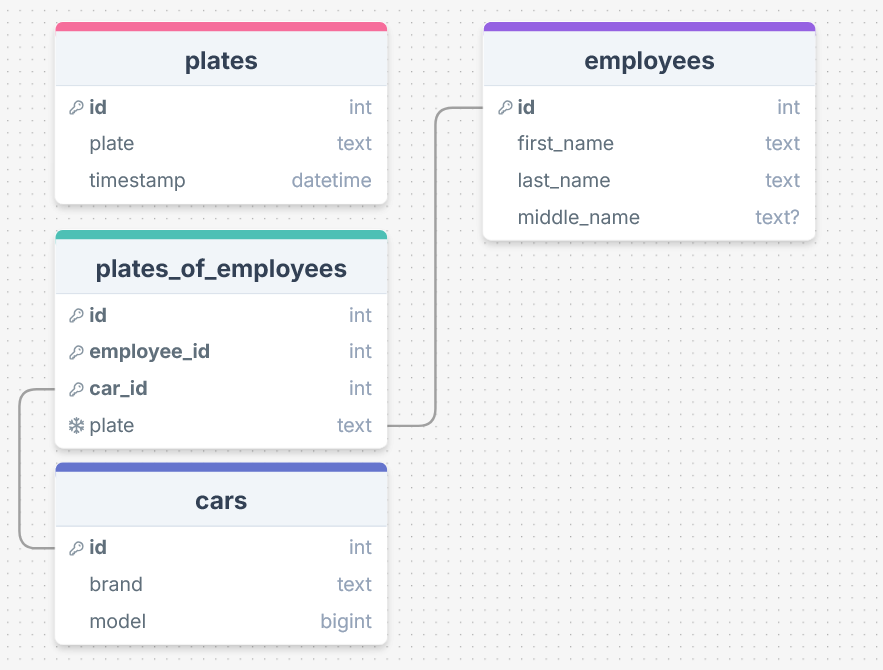
\includegraphics[width=1\linewidth]{db_scheme.png}
    \caption{Схема базы данных}
    \label{fig:enter-label}
\end{figure}

\subsection*{Приложение Б. Примеры обработки видео}

\end{document}